% IEEE conference paper: random-forest transient stability assessment of the IEEE 39-bus system.
% Compile with pdflatex (run twice). Figures are read from ./figures/ (made by make_paper_figures.py).
\documentclass[conference]{IEEEtran}
\IEEEoverridecommandlockouts

\usepackage{cite}
\usepackage{amsmath,amssymb}
\usepackage{graphicx}
\usepackage{booktabs}
\usepackage{textcomp}
\usepackage{xcolor}
\usepackage{tikz}
\usetikzlibrary{positioning,arrows.meta}

\graphicspath{{figures/}}

\begin{document}

\title{Random Forest-Based Transient Stability Assessment of the IEEE 39-Bus System Using Post-Disturbance
Generator Voltage and Frequency Samples}

% TODO: replace the placeholders with the real author names, affiliations and e-mail addresses
\author{\IEEEauthorblockN{First Author}
\IEEEauthorblockA{\textit{Department} \\
\textit{University}\\
City, Country \\
email address}
\and
\IEEEauthorblockN{Second Author}
\IEEEauthorblockA{\textit{Department} \\
\textit{University}\\
City, Country \\
email address}
}

\maketitle

\begin{abstract}
Fast transient stability assessment (TSA) allows operators to act before a disturbed power system loses synchronism.
This paper evaluates a random forest classifier that predicts the transient stability status of the IEEE 39-bus
system from only four post-disturbance samples of the voltage magnitude and frequency at each of the ten generator
buses. The dataset comprises 3715 time-domain simulations of generator trips, line trips, single-line-to-ground,
double-line-to-ground and three-phase-to-ground faults with line tripping, and load disconnections at five loading
levels, labelled with the transient stability index (TSI). To obtain an unbiased estimate, the data are split by
contingency so that no scenario appears in more than one subset, and the forest hyperparameters are selected by
grouped five-fold cross-validation. The selected 300-tree forest reaches a cross-validated balanced accuracy of
$0.942 \pm 0.041$, a validation balanced accuracy of 0.969 and, on an unseen test set, a balanced accuracy of 0.955
with 95.9\,\% of the unstable cases detected and an ROC-AUC of 0.993. The errors concentrate in a few contingencies,
and the forest relies mainly on the frequencies of the two generators that are separated from the network when line
16--19 is lost.
\end{abstract}

\begin{IEEEkeywords}
Transient stability assessment, random forest, machine learning, IEEE 39-bus system, transient stability index.
\end{IEEEkeywords}

%===================================================================================================
\section{Introduction}
%===================================================================================================
Transient stability is the ability of a power system to maintain synchronism after a severe disturbance such as a
short circuit or the loss of a line or generator~\cite{kundur2004}. Time-domain simulation determines the stability
status accurately, but it is too slow to screen many contingencies in real time. Data-driven TSA instead learns the
mapping from a few measurements to the stability status from simulated cases and evaluates it in milliseconds.

Decision trees were among the first learning methods used for on-line dynamic security assessment because their
rules are fast and interpretable~\cite{sun2007}, and rule-based classifiers trained on post-disturbance records have
been shown to predict instability shortly after fault clearing~\cite{kamwa2009}. Ensembles of learners and TSI-based
labelling were combined in~\cite{xu2012}. Random forests~\cite{breiman2001} average many randomised classification
and regression trees~\cite{breiman1984}, which reduces the variance of single trees while keeping their robustness to
feature scaling and outliers.

A common weakness of scenario-based TSA studies is the evaluation protocol: when the same contingency, simulated at
several slightly different loading levels, appears in both the training and the test data, the test score
overestimates performance on unseen contingencies. This paper makes the following contributions:
\begin{itemize}
  \item a random forest that predicts the stability of the IEEE 39-bus system from 80 inputs, namely four voltage and
        four frequency samples at each of the ten generator buses;
  \item a leakage-free evaluation protocol in which the training, validation and test sets as well as the
        cross-validation folds are separated by contingency;
  \item an analysis of the remaining errors by contingency and of the measurements the forest relies on.
\end{itemize}
Section~\ref{sec:data} describes the dataset, Section~\ref{sec:method} the methodology, Section~\ref{sec:results} the
results and Section~\ref{sec:discussion} their implications.

%===================================================================================================
\section{Dataset and Problem Formulation}
\label{sec:data}
%===================================================================================================
\subsection{Test System and Scenarios}
The IEEE 39-bus (New England) system~\cite{athay1979} with ten generators at buses 30--39 was simulated in the time
domain. % TODO: name the simulation tool and the sampling instants of the four samples
Four contingency families were applied (Table~\ref{tab:scenarios}): generator trips, line trips, ground faults on a
line followed by tripping of that line, and load disconnections. Ground faults were single-line-to-ground (SLG),
double-line-to-ground (LLG) or three-phase-to-ground (3PHG), located at 20\,\% or 80\,\% of the line length; faults and
line trips were cleared after 0.1, 0.3 or 0.5\,s. All 34 transmission lines were covered, and every contingency was
simulated at five operating conditions with the system load changed by $-4$, $-2$, 0, $+2$ and $+4$\,\%.

\begin{table}[t]
\caption{Simulated contingencies (each at five load levels)}
\label{tab:scenarios}
\centering
\begin{tabular}{lrrr}
\toprule
Contingency type & Contingencies & Cases & Unstable (\%) \\
\midrule
Generator trip           & 10  & 50   & 10.0 \\
Ground fault + line trip & 612 & 3060 & 15.0 \\
\quad SLG                & 204 & 1020 & 2.9 \\
\quad LLG                & 204 & 1020 & 7.1 \\
\quad 3PHG               & 204 & 1020 & 34.9 \\
Line trip                & 102 & 510  & 41.8 \\
Load disconnection       & 19  & 95   & 0.0 \\
\midrule
Total                    & 743 & 3715 & 18.2 \\
\bottomrule
\end{tabular}
\end{table}

\subsection{Inputs and Stability Label}
For each generator bus B30--B39 the voltage magnitude (p.u.) and the frequency (Hz) are sampled four times after the
disturbance, giving an input vector $\mathbf{x} \in \mathbb{R}^{80}$. The label follows from the transient stability
index~\cite{xu2012}
\begin{equation}
  \mathrm{TSI} = \frac{360^\circ - \Delta\delta_{\max}}{360^\circ + \Delta\delta_{\max}} \times 100,
  \label{eq:tsi}
\end{equation}
where $\Delta\delta_{\max}$ is the maximum rotor-angle separation between any two generators during the simulation; a
case is stable ($y = 1$) if $\mathrm{TSI} > 0$ and unstable ($y = 0$) otherwise.
% TODO: confirm that Eq. (1) is the TSI definition used to label the simulations
Of the 3715 cases, 676 (18.2\,\%) are unstable.

\subsection{Data Characteristics}
Fault duration is the dominant driver of instability (Fig.~\ref{fig:faulttime}): with 0.1-s clearing only 2.9\,\% of
the cases are unstable for every fault kind, whereas 68.8\,\% of the 3PHG faults and 78.2\,\% of the line trips cleared
after 0.5\,s are unstable. The unstable 0.1-s cases are exactly the contingencies on line 16--19, whose loss
disconnects buses 19, 20, 33 and 34, and with them the generators at B33 and B34, from the rest of the network; all 105
cases on this line are unstable. A heavier load raises the unstable share from 13.9\,\% at $-4$\,\% to 22.5\,\% at
$+4$\,\%, and all 64 contingencies whose label changes with the load change from stable to unstable as the load
increases. Unstable cases show depressed voltages and over-frequencies at the generator buses (Fig.~\ref{fig:traces}).

\begin{figure}[t]
  \centering
  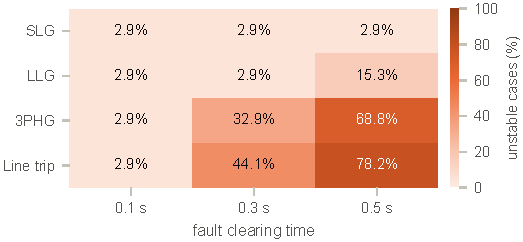
\includegraphics[width=\columnwidth]{fig_fault_time.pdf}
  \caption{Share of unstable cases by fault kind and clearing time.}
  \label{fig:faulttime}
\end{figure}

\begin{figure}[t]
  \centering
  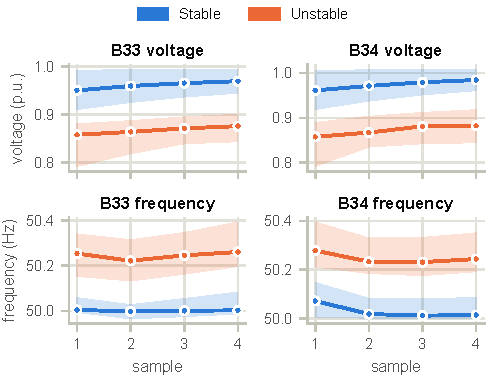
\includegraphics[width=\columnwidth]{fig_traces.pdf}
  \caption{Voltage and frequency at B33 and B34 over the four samples (line: median, band: interquartile range).}
  \label{fig:traces}
\end{figure}

\subsection{Data Quality}
The dataset has no missing or duplicate values. Ten cases contain physically impossible readings (voltages of
9--13\,p.u.\ and frequencies between 24 and 81\,Hz at B33 and B34). All of them are 3PHG faults on line 16--19 cleared
after 0.3 or 0.5\,s, i.e.\ two contingencies at five load levels, and all are unstable. They stem from the large
fluctuations of the generators that lose synchronism and are retained in this study.

%===================================================================================================
\section{Methodology}
\label{sec:method}
%===================================================================================================
The procedure is summarised in Fig.~\ref{fig:flow}.

\begin{figure}[t]
\centering
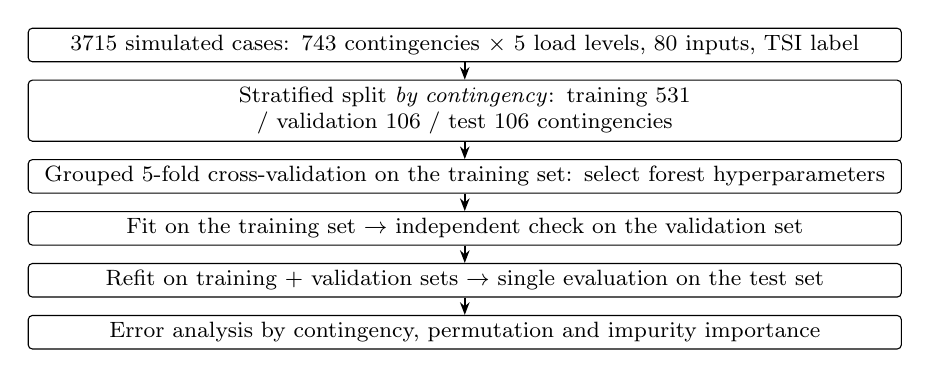
\begin{tikzpicture}[node distance=2.2mm, every node/.style={font=\footnotesize},
  box/.style={draw, rounded corners=1.5pt, align=center, text width=0.9\columnwidth, inner sep=2.5pt},
  arr/.style={-{Stealth[length=1.6mm]}, thick}]
  \node[box] (a) {3715 simulated cases: 743 contingencies $\times$ 5 load levels, 80 inputs, TSI label};
  \node[box, below=of a] (b) {Stratified split \emph{by contingency}: training 531 / validation 106 / test 106 contingencies};
  \node[box, below=of b] (c) {Grouped 5-fold cross-validation on the training set: select forest hyperparameters};
  \node[box, below=of c] (d) {Fit on the training set $\rightarrow$ independent check on the validation set};
  \node[box, below=of d] (e) {Refit on training + validation sets $\rightarrow$ single evaluation on the test set};
  \node[box, below=of e] (f) {Error analysis by contingency, permutation and impurity importance};
  \draw[arr] (a) -- (b); \draw[arr] (b) -- (c); \draw[arr] (c) -- (d); \draw[arr] (d) -- (e); \draw[arr] (e) -- (f);
\end{tikzpicture}
\caption{Training and evaluation procedure.}
\label{fig:flow}
\end{figure}

\subsection{Contingency-Grouped Data Split}
Each contingency appears five times, once per load level, and these cases are nearly identical. The data are therefore
split by contingency with a stratified group split, so that all load levels of a contingency fall into the same subset
and each subset keeps the same share of unstable cases (Table~\ref{tab:split}). The two contingencies containing the
impossible readings are assigned to the training set, so that the model is trained with them. No contingency is
shared between subsets.

\begin{table}[t]
\caption{Training, validation and test sets}
\label{tab:split}
\centering
\begin{tabular}{lrrrr}
\toprule
Set & Cases & Contingencies & Unstable & Unstable (\%) \\
\midrule
Training   & 2655 & 531 & 483 & 18.2 \\
Validation & 530  & 106 & 96  & 18.1 \\
Test       & 530  & 106 & 97  & 18.3 \\
\bottomrule
\end{tabular}
\end{table}

\subsection{Random Forest Classifier}
A random forest~\cite{breiman2001} is an ensemble of $T$ classification trees~\cite{breiman1984}. Each tree is grown
on a bootstrap sample of the training cases. At every node, $m$ randomly chosen inputs are examined, and the split
that most reduces the weighted Gini impurity
\begin{equation}
  G = 1 - \sum_{k \in \{0,1\}} p_k^2, \qquad p_k = \frac{\sum_{i \in \text{node},\, y_i = k} w_{y_i}}{\sum_{i \in \text{node}} w_{y_i}},
\end{equation}
is selected. The class weights $w_k = n/(2 n_k)$, where $n_k$ is the number of training cases of class $k$, compensate
for the class imbalance; an unstable case weighs about 4.5 times as much as a stable one. The forest estimates the
probability of instability as the average of the tree estimates,
\begin{equation}
  \hat{P}(\text{unstable} \mid \mathbf{x}) = \frac{1}{T} \sum_{t=1}^{T} \hat{p}_t(\text{unstable} \mid \mathbf{x}),
\end{equation}
and a case is classified as unstable when $\hat{P} \ge 0.5$. Because trees split on thresholds, the inputs need no
scaling. The forest uses $T = 300$ trees.

\subsection{Hyperparameter Selection}
The maximum tree depth (unlimited, 16 or 8), the minimum number of cases per leaf (1, 3 or 10), the share of inputs
examined per split ($\sqrt{80} \approx 9$ inputs, 30\,\% or 60\,\%) and the class weighting (computed on the whole
training set or per bootstrap sample) were searched on a full grid of 54 combinations. Each combination was scored by
grouped five-fold cross-validation inside the training set: the 531 training contingencies are divided into five
folds, each fold is held out once, and the mean balanced accuracy is used for selection.

\subsection{Evaluation Metrics}
The unstable class is the positive class. With TP, FN, FP and TN the counts of unstable cases detected and missed and of
stable cases falsely flagged and correctly classified, the balanced accuracy is
$\mathrm{BA} = \tfrac{1}{2}\left[\mathrm{TP}/(\mathrm{TP}+\mathrm{FN}) + \mathrm{TN}/(\mathrm{TN}+\mathrm{FP})\right]$.
The unstable recall $\mathrm{TP}/(\mathrm{TP}+\mathrm{FN})$, the precision $\mathrm{TP}/(\mathrm{TP}+\mathrm{FP})$ and the
area under the ROC curve (ROC-AUC) of $\hat{P}$ are also reported. The models were implemented with
scikit-learn~\cite{pedregosa2011}.

%===================================================================================================
\section{Results}
\label{sec:results}
%===================================================================================================
\subsection{Hyperparameter Selection}
Fig.~\ref{fig:cvgrid} shows the cross-validated balanced accuracy for the balanced class weighting, which outperformed
per-bootstrap weighting (0.930--0.942 versus 0.913--0.935). The best setting uses 30\,\% of the inputs per split and at
least 10 cases per leaf, with a balanced accuracy of $0.942 \pm 0.041$. The depth limit has no effect, because the
trees stop growing before reaching it, and the whole balanced-weight grid lies within 0.012, so the forest is
insensitive to its hyperparameters. The standard deviation of 0.041 between folds shows that the difficulty depends
strongly on which contingencies are held out.

\begin{figure}[t]
  \centering
  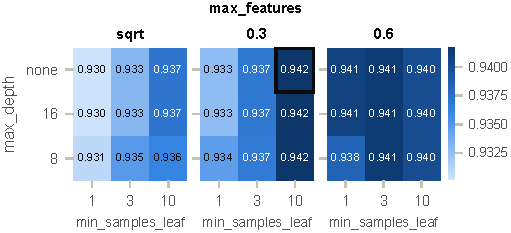
\includegraphics[width=\columnwidth]{fig_cv_grid.pdf}
  \caption{Cross-validated balanced accuracy (balanced class weights). Panels: share of inputs per split; box:
  selected setting.}
  \label{fig:cvgrid}
\end{figure}

\subsection{Classification Performance}
Table~\ref{tab:results} summarises the results. Fitted on the training set, the forest reaches a balanced accuracy of
0.969 on the validation set and detects 93 of 96 unstable cases with 13 false alarms. Refitted on the training and
validation sets and evaluated once on the test set, it reaches a balanced accuracy of 0.955, detects 93 of 97 unstable
cases (95.9\,\%) and raises 21 false alarms among 433 stable cases (Fig.~\ref{fig:cm}). The ROC-AUC is 0.997 on the
validation set and 0.993 on the test set (Fig.~\ref{fig:roc}). On the test set all generator trips and load
disconnections are classified correctly, ground faults with 96.3\,\% and line trips with 88.8\,\% accuracy, and the
accuracy at each load level lies between 92.5 and 97.2\,\%.

A learning curve on the validation set shows a balanced accuracy of 0.88 with up to 1060 training cases, which rises
to 0.95--0.97 with 1595 or more cases, while the training score stays at 0.99. Additional scenarios of the same kind
would therefore bring only small gains.

\begin{table}[t]
\caption{Classification results (unstable = positive class)}
\label{tab:results}
\centering
\setlength{\tabcolsep}{4pt}
\begin{tabular}{lrrrrr}
\toprule
Set & BA & Recall & Precision & Stable rec. & ROC-AUC \\
\midrule
CV (training)  & 0.942 & -- & -- & -- & -- \\
Training       & 0.989 & 0.998 & 0.918 & 0.980 & 1.000 \\
Validation     & 0.969 & 0.969 & 0.877 & 0.970 & 0.997 \\
Test           & \textbf{0.955} & \textbf{0.959} & \textbf{0.816} & \textbf{0.952} & \textbf{0.993} \\
\bottomrule
\end{tabular}
\end{table}

\begin{figure}[t]
  \centering
  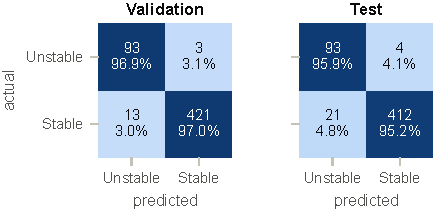
\includegraphics[width=\columnwidth]{fig_confusion.pdf}
  \caption{Confusion matrices: validation (forest fitted on the training set) and test (final forest).}
  \label{fig:cm}
\end{figure}

\begin{figure}[t]
  \centering
  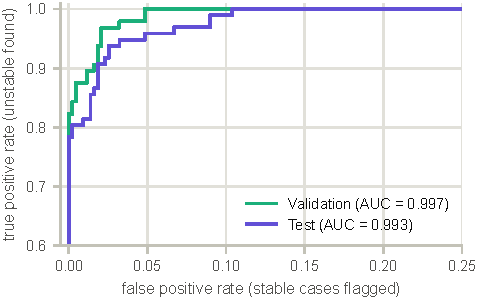
\includegraphics[width=\columnwidth]{fig_roc.pdf}
  \caption{ROC curves on the validation and test sets (zoomed to the upper-left corner).}
  \label{fig:roc}
\end{figure}

\subsection{Error Analysis}
The 25 test errors come from 13 contingencies (Table~\ref{tab:errors}). All four missed unstable cases are 3PHG faults
on line 28--29 cleared after 0.5\,s, with predicted probabilities of 0.21--0.46. Ten of the 21 false alarms come from
two contingencies that are misclassified at all five load levels: an LLG fault on line 16--17 cleared after 0.5\,s
($\hat{P} = 0.57$--$0.66$) and the trip of line 22--23 after 0.3\,s ($\hat{P} = 0.73$--$0.84$). The other false alarms are
severe faults and line trips with 0.3--0.5\,s clearing, i.e.\ survivable disturbances close to the stability
boundary. On the validation set, the three missed cases are 0.5-s trips of lines 2--3 and 2--25 with
$\hat{P} = 0.38$--$0.49$, just below the threshold.

\begin{table}[t]
\caption{Test errors grouped by contingency}
\label{tab:errors}
\centering
\setlength{\tabcolsep}{3.5pt}
\begin{tabular}{llrl}
\toprule
Contingency & Error & Cases & $\hat{P}$(unstable) \\
\midrule
3PHG line 28--29, 80\,\%, 0.5\,s & missed & 3 & 0.21--0.46 \\
3PHG line 28--29, 20\,\%, 0.5\,s & missed & 1 & 0.29 \\
LLG line 16--17, 20\,\%, 0.5\,s  & false alarm & 5 & 0.57--0.66 \\
Line trip 22--23, 0.3\,s        & false alarm & 5 & 0.73--0.84 \\
3PHG line 16--17, 80\,\%, 0.3\,s & false alarm & 2 & 0.59--0.67 \\
3PHG line 21--22, 20\,\%, 0.3\,s & false alarm & 2 & 0.54--0.58 \\
Seven other contingencies       & false alarm & 7 & 0.54--0.80 \\
\bottomrule
\end{tabular}
\end{table}

\subsection{Feature Importance}
Fig.~\ref{fig:importance} shows two importance measures, each summed over the four samples of a bus quantity. The
permutation importance, i.e.\ the drop in test balanced accuracy when the samples are shuffled across cases, is
dominated by the frequencies at B34 (0.128) and B33 (0.104), followed at a distance by the B39 frequency (0.021). The
impurity importance, accumulated during training, confirms this ranking: the B34 and B33 frequencies account for
0.371 and 0.276 of the total Gini decrease. B33 and B34 are the generators that are disconnected from the network
when line 16--19 is lost, and the frequency of an islanded generator departs quickly from that of the main system.
Because impurity importance is computed on training data and can favour inputs with many distinct
values~\cite{strobl2007}, the permutation importance on the test set is the more reliable of the two.

\begin{figure}[t]
  \centering
  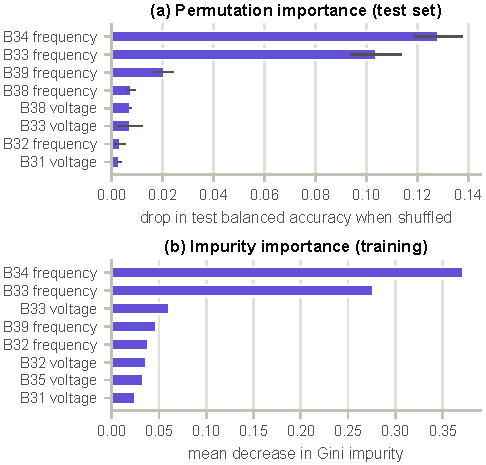
\includegraphics[width=\columnwidth]{fig_importance.pdf}
  \caption{Feature importance of the final forest, summed over the four samples of each bus voltage and frequency
  (top eight).}
  \label{fig:importance}
\end{figure}

%===================================================================================================
\section{Discussion}
\label{sec:discussion}
%===================================================================================================
The three performance estimates (cross-validation 0.942, validation 0.969, test 0.955) differ by up to 2.7 points
because each held-out set contains only about 106 contingencies and the errors cluster in a few of them. The
cross-validated standard deviation of 0.041 shows the same effect; a realistic expectation for unseen contingencies of
the simulated kinds is a balanced accuracy of about 0.94--0.97. Splitting by contingency is essential for this
estimate, since the five load levels of a contingency would otherwise appear on both sides of the split.

The ten impossible readings were kept in the training data. Because tree splits depend only on the ordering of the
values, such readings cannot distort the model the way they can affect distance-based learners, and inputs outside the
training range simply fall into the outermost branch of each split. The strong reliance on the B33 and B34 frequencies
reflects the islanding of these generators after the loss of line 16--19, which accounts for 105 of the 676 unstable
cases; contingencies that destabilise other parts of the system, such as the 3PHG faults on line 28--29, are
the ones the forest still misses. Lowering the 0.5 decision threshold would trade more false alarms for fewer missed
unstable cases.

The study is limited to simulated data of one test system and one set of operating conditions, only ten
generator-trip contingencies are available, and the four samples cover only the early post-disturbance period, so
instability that develops later leaves little trace in the inputs.

%===================================================================================================
\section{Conclusion}
%===================================================================================================
A random forest using only four voltage and four frequency samples from each of the ten generators of the IEEE 39-bus
system predicts transient stability with a balanced accuracy of 0.955 on unseen test contingencies, detecting 95.9\,\%
of the unstable cases with an ROC-AUC of 0.993. A contingency-grouped split and grouped cross-validation give an
unbiased estimate of this performance. The forest is insensitive to its hyperparameters, needs no input scaling and
relies mainly on the frequencies of the generators separated by the loss of line 16--19. Future work will examine the
removal or capping of the impossible readings, a tuned decision threshold, more diverse generator-trip scenarios and
engineered inputs such as the frequency spread between generators.

% TODO: verify reference details (authors, volume, pages) before submission
\begin{thebibliography}{00}
\bibitem{kundur2004} P. Kundur \textit{et al.}, ``Definition and classification of power system stability,''
\textit{IEEE Trans. Power Syst.}, vol. 19, no. 3, pp. 1387--1401, Aug. 2004.
\bibitem{athay1979} T. Athay, R. Podmore, and S. Virmani, ``A practical method for the direct analysis of transient
stability,'' \textit{IEEE Trans. Power App. Syst.}, vol. PAS-98, no. 2, pp. 573--584, Mar. 1979.
\bibitem{breiman2001} L. Breiman, ``Random forests,'' \textit{Mach. Learn.}, vol. 45, no. 1, pp. 5--32, 2001.
\bibitem{breiman1984} L. Breiman, J. H. Friedman, R. A. Olshen, and C. J. Stone, \textit{Classification and Regression
Trees}. Belmont, CA, USA: Wadsworth, 1984.
\bibitem{sun2007} K. Sun, S. Likhate, V. Vittal, V. S. Kolluri, and S. Mandal, ``An online dynamic security assessment
scheme using phasor measurements and decision trees,'' \textit{IEEE Trans. Power Syst.}, vol. 22, no. 4,
pp. 1935--1943, Nov. 2007.
\bibitem{kamwa2009} I. Kamwa, S. R. Samantaray, and G. Joos, ``Development of rule-based classifiers for rapid
stability assessment of wide-area post-disturbance records,'' \textit{IEEE Trans. Power Syst.}, vol. 24, no. 1,
pp. 258--270, Feb. 2009.
\bibitem{xu2012} Y. Xu, Z. Y. Dong, J. H. Zhao, P. Zhang, and K. P. Wong, ``A reliable intelligent system for real-time
dynamic security assessment of power systems,'' \textit{IEEE Trans. Power Syst.}, vol. 27, no. 3, pp. 1253--1263,
Aug. 2012.
\bibitem{strobl2007} C. Strobl, A.-L. Boulesteix, A. Zeileis, and T. Hothorn, ``Bias in random forest variable
importance measures: Illustrations, sources and a solution,'' \textit{BMC Bioinformatics}, vol. 8, art. 25, 2007.
\bibitem{pedregosa2011} F. Pedregosa \textit{et al.}, ``Scikit-learn: Machine learning in Python,''
\textit{J. Mach. Learn. Res.}, vol. 12, pp. 2825--2830, 2011.
\end{thebibliography}

\end{document}
